\chapter{线性算子方程}
\label{chap:linear-operator-equations}

前几章大多在正向使用算子：给定输入函数，计算积分、投影或微分得到输出。许多问题却是反过来的。测得一个经过平均的信号，要推回产生它的输入；或者未知函数同时出现在积分号内外，要从源项把它解出来。于是要问三件事：给定的输出能否由某个输入产生，产生它的输入是否唯一，输出中的小误差会不会在解中变成大误差。

本章在Hilbert空间中研究这三个问题。第~\ref{sec:opeq-first-kind}节处理第一类方程$Kf=g$：它是否有解取决于$g$是否落在$K$的像中，是否唯一取决于零空间；第~\ref{chap:operator-spectra}章的奇异系统把这两个条件改写成系数条件，并说明“$g$能被输出任意逼近”还不等于“方程有解”。第~\ref{sec:opeq-second-kind}节处理第二类方程$(I-\lambda K)u=f$。恒等项使这类方程的结构完全不同：参数较小时可以用Neumann级数直接构造逆，一般参数下由Fredholm择一给出只含有限个约束的可解条件。

第~\ref{sec:opeq-stability}节把可解与唯一之外的第三个问题单独拿出来：固定输入输出的范数之后，解是否连续依赖于数据。第一类紧算子方程的像不闭，趋于零的奇异值把数据误差无界地放大；第二类方程只在参数接近共振值时变得敏感。全章用两个小算子作贯穿例子：$L^2([-1,1])$上核为$1+xz$的秩二积分算子，以及$L^2(0,1)$上的积分算子$(Vf)(x)=\int_0^xf$。

本章只回答方程何时可解、解怎样依赖数据，以及形式逆为什么不能直接使用。怎样选择截断位置或惩罚强度、怎样在偏差与误差放大之间取舍并设计求解算法，属于卷五的正则化问题；矩阵方程的直接解法与迭代解法已在卷二讨论。

\section{第一类算子方程}
\label{sec:opeq-first-kind}

测量仪器往往不直接给出我们想知道的函数，而是给出它经过平均、平滑或累积后的结果。若这个过程是线性的，就可以写成一个算子$K$作用在未知函数$f$上，测得的输出是$g$。从$g$推回$f$，就是求解一个算子方程。本节固定Hilbert空间之间的紧算子，先说明“有解”和“唯一”分别对应算子的哪个对象，再借助奇异系统把这两个条件写成可以逐项核对的系数条件。

\paragraph{方程与两个基本问题}
设$H_1,H_2$是同一数域$\mathbb F$（$\mathbb R$或$\mathbb C$）上的Hilbert空间，$K\in\mathcal B(H_1,H_2)$，$g\in H_2$已知。复内积沿用对第一个变量共轭线性、对第二个变量线性的约定。

\begin{definition}[第一类算子方程]
\label{def:opeq-first-kind}
给定$K\in\mathcal B(H_1,H_2)$与$g\in H_2$，求$f\in H_1$使
\begin{equation}
  Kf=g ,
  \label{eq:opeq-first-kind}
\end{equation}
称为\term{第一类算子方程}（operator equation of the first kind）。$K$为积分算子时，也称为第一类积分方程。
\end{definition}

这里未知函数只出现在算子里面，方程等于问：$g$是不是$K$的一个输出。由此立即得到两条判别。方程~\eqref{eq:opeq-first-kind}有解当且仅当$g\in\operatorname{Ran}K$。若$f_0$是一个解，则$f$是解当且仅当$K(f-f_0)=0$，所以全部解组成$f_0+\ker K$；解唯一当且仅当$\ker K=\{0\}$。存在性问的是输出空间里的一个集合，唯一性问的是输入空间里的一个子空间，两者需要分别核对。

\paragraph{秩二积分算子的例子}
取$H=L^2([-1,1],\mu)$，其中$\mathrm d\mu=\mathrm dz/2$，在其上定义核为$1+xz$的积分算子
\begin{equation}
  (Tf)(x)=\int_{-1}^{1}(1+xz)f(z)\,\frac{\mathrm dz}2
  =\langle 1,f\rangle+x\,\langle z,f\rangle ,
  \label{eq:opeq-rank-two}
\end{equation}
这里核是实值的，$\langle 1,f\rangle$与$\langle z,f\rangle$分别是$f$与常函数$1$、一次函数$z$的内积。在这个测度下$\lVert1\rVert^2=1$，$\lVert x\rVert^2=\int_{-1}^1x^2\,\mathrm dx/2=1/3$，而$\langle1,x\rangle=0$。于是任意$f$可以唯一地写成$f=\alpha+\beta x+h$，其中$h$与$1,x$都正交，代入得
\[
  Tf=\alpha+\frac{\beta}{3}x .
\]
$T$的像是二维子空间$\operatorname{span}\{1,x\}$，零空间是$\{1,x\}$的正交补，后者是无限维的；例如$x^2-1/3$就在其中，因为它与$1$和$x$都正交。

因此第一类方程$Tf=g$只在$g=a+bx$时有解。比较系数得$\alpha=a$、$\beta=3b$，而$h$完全不受约束：
\[
  f=a+3bx+h,\qquad h\perp1,\ h\perp x .
\]
解一旦存在就有无穷多个，差别正是零空间中的任意元素。若$g$含有$x^2$这样的成分，无论怎样选$f$都得不到$g$：$T$把与$1,x$正交的方向全部压成零，这些方向上的信息在输出中已经丢失。

\paragraph{奇异系统下的系数关系}
对一般的紧算子，像和零空间不再这样一目了然。第~\ref{chap:operator-spectra}章为两个Hilbert空间之间的紧算子$K$构造了奇异系统：正数$\sigma_1\geq\sigma_2\geq\cdots>0$（有限个或可数无穷个，后者有$\sigma_j\to0$），$H_1$中的标准正交系$(v_j)$与$H_2$中的标准正交系$(u_j)$，使
\begin{equation}
  Kx=\sum_j\sigma_j\langle v_j,x\rangle u_j ,\qquad K^*u_j=\sigma_jv_j ,
  \label{eq:opeq-svd}
\end{equation}
并且$(v_j)$的闭线性张成是$(\ker K)^\perp$，$(u_j)$的闭线性张成是$\overline{\operatorname{Ran}K}$。第~\ref{chap:linear-operators}章又给出$\overline{\operatorname{Ran}K}=(\ker K^*)^\perp$。下面只用到这几条结论。

若$Kf=g$，对每个$j$取$u_j$与方程两边作内积，并把$K$移到另一侧：
\[
  \langle u_j,g\rangle=\langle u_j,Kf\rangle=\langle K^*u_j,f\rangle=\sigma_j\langle v_j,f\rangle .
\]
解在方向$v_j$上的系数因此被数据唯一确定为$\langle u_j,g\rangle/\sigma_j$。这一关系把方程拆成了可数个标量方程，但也提出了一个新要求：这些系数必须平方可和，拼起来的级数才代表$H_1$中的元素。

\begin{theorem}[第一类方程的可解条件与最小范数解]
\label{thm:opeq-picard}
设$K:H_1\to H_2$为紧算子，奇异系统如式~\eqref{eq:opeq-svd}。方程$Kf=g$有解，当且仅当以下两条同时成立：
\begin{equation}
  g\perp\ker K^* ,\qquad
  \sum_j\frac{\lvert\langle u_j,g\rangle\rvert^2}{\sigma_j^2}<\infty .
  \label{eq:opeq-picard}
\end{equation}
此时
\[
  f^\dagger=\sum_j\frac{\langle u_j,g\rangle}{\sigma_j}v_j
\]
是方程在$(\ker K)^\perp$中唯一的解，全部解为$f^\dagger+\ker K$，并且$f^\dagger$是范数最小的解。
\end{theorem}

\begin{proof}
必要性。若$Kf=g$，则$g\in\operatorname{Ran}K\subseteq(\ker K^*)^\perp$，第一条成立。由上面的系数关系和Bessel不等式，
\[
  \sum_j\frac{\lvert\langle u_j,g\rangle\rvert^2}{\sigma_j^2}=\sum_j\lvert\langle v_j,f\rangle\rvert^2\leq\lVert f\rVert^2<\infty ,
\]
第二条成立。

充分性。第二条说明$f^\dagger$的系数平方可和，所以级数在$H_1$中按范数收敛，且$f^\dagger$属于$(v_j)$的闭张成$(\ker K)^\perp$。$K$连续，可以逐项作用；由$Kv_j=\sigma_ju_j$得
\[
  Kf^\dagger=\sum_j\langle u_j,g\rangle u_j ,
\]
这是$g$在$(u_j)$的闭张成上的正交投影。这个闭张成等于$\overline{\operatorname{Ran}K}=(\ker K^*)^\perp$，第一条说明$g$就在其中，所以投影等于$g$本身，即$Kf^\dagger=g$。

解的结构。全部解为$f^\dagger+\ker K$。若$f_1,f_2$都是$(\ker K)^\perp$中的解，则$f_1-f_2$同时属于$\ker K$与$(\ker K)^\perp$，只能为零。对任意解$f=f^\dagger+h$，$h\in\ker K$与$f^\dagger$正交，由勾股定理$\lVert f\rVert^2=\lVert f^\dagger\rVert^2+\lVert h\rVert^2\geq\lVert f^\dagger\rVert^2$。
\end{proof}

式~\eqref{eq:opeq-picard}中的第二个条件称为\term{Picard条件}（Picard condition），$f^\dagger$称为方程的最小范数解。两个条件分工不同。第一个只说明$g$落在像的闭包里，也就是$g$能被输出任意逼近；第二个才保证形式上的逆系数真正拼成输入空间中的元素。$K$只有有限个正奇异值时，第二个条件自动成立，只剩第一个；在秩二的例子中，$T$自伴且奇异值为$1$与$1/3$，对$g=a+bx$得$f^\dagger=a+3bx$，正是全部解中零空间分量为零的那一个。

\paragraph{像的闭包不等于像}
奇异值无限多时，两个条件确实不同。最简单的例子是$\ell^2$上的对角算子$A(x_n)=(x_n/n)$。它自伴、单射，$\ker A^*=\{0\}$，第一个条件对所有数据成立；奇异值为$1/n$，Picard条件化为$\sum_nn^2\lvert g_n\rvert^2<\infty$。取$g^{(1)}_n=1/n^2$，形式解系数为$1/n$，平方可和，方程有解$(1/n)$。取$g^{(2)}_n=1/n$，它本身平方可和，形式解系数却恒为$1$，所以$g^{(2)}$不在像中。图~\ref{fig:opeq-picard-coefficients}比较了这两组数据。

\begin{figure}[!htb]
  \centering
  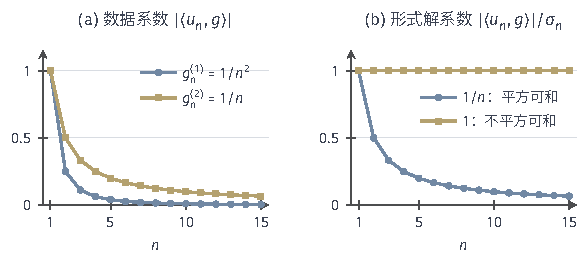
\includegraphics[width=99.6mm]{figures/02-abstract-mathematics/03-function-spaces/tikz/c3-picard-coefficients/figure.pdf}
  \caption{$\ell^2$上$A(x_n)=(x_n/n)$的Picard条件。(a)两组数据的系数$1/n^2$与$1/n$，都平方可和，都与$\ker A^*=\{0\}$正交。(b)除以奇异值$\sigma_n=1/n$后的形式解系数：前者为$1/n$，平方可和，方程可解；后者恒为$1$，不平方可和，方程无解。}
  \label{fig:opeq-picard-coefficients}
\end{figure}

函数空间中有同样的现象。在$L^2(0,1)$上考虑累积积分
\[
  (Vf)(x)=\int_0^xf(t)\,\mathrm dt .
\]
由Fubini定理交换积分次序，
\begin{equation*}
\langle g,Vf\rangle=\int_0^1\overline{g(x)}\int_0^xf(t)\,\mathrm dt\,\mathrm dx=\int_0^1\Bigl(\int_t^1\overline{g(x)}\,\mathrm dx\Bigr)f(t)\,\mathrm dt,
\end{equation*}
所以伴随为$(V^*g)(t)=\int_t^1g(x)\,\mathrm dx$。若$Vf=0$，则$f$在每个区间$[0,x]$上的积分为零，从而在每个子区间上的积分为零，$f=0$几乎处处；同理$V^*$也是单射。于是$\ker V=\ker V^*=\{0\}$，$V$的像在$L^2(0,1)$中稠密。

$V$的奇异系统可以直接写出。记$\omega_k=(k-\frac12)\pi$，$k=1,2,\ldots$，令
\[
  v_k(x)=\sqrt2\cos\omega_kx,\qquad u_k(x)=\sqrt2\sin\omega_kx,\qquad \sigma_k=\frac1{\omega_k}.
\]
直接积分得$Vv_k=\sqrt2\sin(\omega_kx)/\omega_k=\sigma_ku_k$；又由$\cos\omega_k=0$，$V^*u_k=\sqrt2\bigl(\cos\omega_kx-\cos\omega_k\bigr)/\omega_k=\sigma_kv_k$。由$\sin2\omega_k=0$可验证$(v_k)$与$(u_k)$各自标准正交。

还要说明这些就是全部奇异方向。$V^*V$是紧自伴算子且为单射，由第~\ref{chap:operator-spectra}章的谱分解，它的非零特征方向张成整个$L^2(0,1)$。若$V^*Vf=\mu f$，$\mu>0$，令$y=V^*Vf$，则$y(x)=\int_x^1\int_0^tf$，于是$y(1)=0$，$y'(x)=-\int_0^xf$，$y'(0)=0$。$f=y/\mu$连续，故$y$二阶连续可微且$y''=-f=-y/\mu$。满足$y'(0)=0$的解为$y=c\cos(x/\sqrt\mu)$，再由$y(1)=0$得$1/\sqrt\mu=\omega_k$。因此特征值为$\sigma_k^2$，每个特征空间由$v_k$张成，$(v_k)$是$L^2(0,1)$的标准正交基。

现在取数据$g=1$。由$\ker V^*=\{0\}$，它满足第一个条件。系数为
\[
  \langle u_k,1\rangle=\sqrt2\int_0^1\sin\omega_kx\,\mathrm dx=\frac{\sqrt2(1-\cos\omega_k)}{\omega_k}=\sqrt2\,\sigma_k ,
\]
形式解系数恒为$\sqrt2$，Picard条件不成立，所以$1\notin\operatorname{Ran}V$。这与直接观察一致：$Vf$总有在$0$处取零的连续代表，而常函数$1$的连续代表在$0$处取$1$，两个连续函数若几乎处处相等就处处相等。

$1$能被输出逼近，逼近的代价是输入越来越大。取$f_n=n\mathbf 1_{[0,1/n]}$，则$(Vf_n)(x)=\min\{nx,1\}$，
\[
  \lVert Vf_n-1\rVert^2=\int_0^{1/n}(1-nx)^2\,\mathrm dx=\frac1{3n}\to0,\qquad \lVert f_n\rVert^2=n\to\infty .
\]
输出误差趋于零时，产生这些输出的输入并不收敛，它们的范数无界。像的闭包里多出来的元素，正是只能这样“追到”而不能真正达到的数据。

\paragraph{Picard条件与求导}
对一般数据，$V$的Picard条件有一个熟悉的含义。设$g$有绝对连续的代表，$g(0)=0$且$g'\in L^2(0,1)$。分部积分，并利用$\cos\omega_k=0$与$g(0)=0$消去边界项：
\[
  \langle u_k,g\rangle=\Bigl[-\frac{\sqrt2\cos\omega_kx}{\omega_k}g(x)\Bigr]_0^1+\frac1{\omega_k}\int_0^1\sqrt2\cos(\omega_kx)\,g'(x)\,\mathrm dx=\sigma_k\langle v_k,g'\rangle .
\]
这里$g$取实值；复值时对实部、虚部分别计算即可。于是Picard级数等于$\sum_k\lvert\langle v_k,g'\rangle\rvert^2=\lVert g'\rVert^2<\infty$，最小范数解就是$f^\dagger=g'$。反过来，若$Vf=g$，则$g$绝对连续、$g(0)=0$且$g'=f$几乎处处。所以$\operatorname{Ran}V$恰好由这样的函数组成，求解第一类方程$Vf=g$就是对数据求导。

这个例子把前面的两个条件落到了具体的函数性质上：$g\perp\ker V^*$对所有$L^2$函数成立，几乎不提供信息；Picard条件则要求数据在$0$处的值合适并具有平方可积的导数。数据的这种正则性正是由奇异值趋于零的速度决定的，它将在第~\ref{sec:opeq-stability}节中重新出现，成为误差放大的来源。

\section{第二类算子方程}
\label{sec:opeq-second-kind}

另一类方程中，未知函数同时出现在算子里面和外面：$u$等于已知的源项加上$u$自身的一个积分平均。写成矩阵，就是$(\bm I-\lambda\bm A)\bm x=\bm b$。多出来的这个恒等项看起来不起眼，却改变了方程的全部性质。本节先在贯穿例子上比较两类方程，再分两步研究可解性：参数较小时直接构造逆，一般参数下建立Fredholm择一。

\paragraph{方程与恒等项}
设$H$为Hilbert空间，$K:H\to H$为紧算子。与第一类方程不同，这里输入和输出必须在同一个空间中，$u$与$Ku$才能相减。

\begin{definition}[第二类算子方程]
\label{def:opeq-second-kind}
给定紧算子$K:H\to H$、参数$\lambda\in\mathbb F$与$f\in H$，求$u\in H$使
\begin{equation}
  (I-\lambda K)u=f,
  \label{eq:opeq-second-kind}
\end{equation}
称为\term{第二类算子方程}（operator equation of the second kind）。若$K$是核为$k$的积分算子，方程写成
\begin{equation}
  u(x)-\lambda\int k(x,z)u(z)\,\mathrm d\mu(z)=f(x),
  \label{eq:opeq-second-kind-integral}
\end{equation}
也称为第二类积分方程。
\end{definition}

回到秩二算子$T$，它在三类方向上分别乘以$1$、$\frac13$、$0$。把$u=\alpha+\beta x+h$与$f=a+bx+r$按同样的方式分解，$h,r$都与$1,x$正交，逐方向比较系数：
\begin{equation}
  (1-\lambda)\alpha=a,\qquad
  \Bigl(1-\frac\lambda3\Bigr)\beta=b,\qquad
  h=r.
  \label{eq:opeq-rank-two-second}
\end{equation}

只要$\lambda\neq1,3$，每个$f$都给出唯一解。例如$\lambda=\frac12$时，三个方向的结果是
\[
  \alpha=2a,\qquad \beta=\frac65b,\qquad h=r.
\]
第一类方程把正交补方向压成零，信息丢失；这里$I-\lambda T$在这些方向上恰好是恒等作用，信息完好。图~\ref{fig:opeq-equation-types}把这一差别画成各方向上的乘子：蓝色的乘子有零，绿色的没有。

\begin{BookInlineFigure}
  \centering
  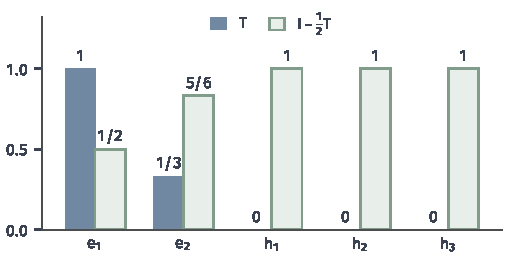
\includegraphics[width=86mm]{figures/04-spaces-measures-and-geometry/03-function-spaces/matplotlib/opeq-equation-types/figure.pdf}
  \caption{核$1+xz$（测度$\mathrm dz/2$）给出的两类方程在各正交方向上的乘子。$e_1=1$、$e_2=\sqrt3x$是特征方向，$h_1,h_2,h_3$代表与它们正交的方向（如$x^2-\frac13$）。蓝色为第一类方程的算子$T$，在正交方向上为零；绿色为第二类方程的算子$I-\frac12T$，在正交方向上恒为$1$。}
  \label{fig:opeq-equation-types}
\end{BookInlineFigure}

困难只出现在两个特殊参数上：$\lambda=1$时齐次方程$(I-T)u=0$有非零解$u=1$，$\lambda=3$时有非零解$u=x$。它们正是特征值$1$与$\frac13$的倒数。

两类方程可以使用同一个积分核，可解性却由整个算子的结构决定。第一类方程的困难来自$K$本身：零空间造成不唯一，像不够大造成无解。第二类方程只在$1/\lambda$恰为$K$的特征值时出问题。下面两个小节分别处理“$\lambda$足够小”与“$\lambda$任意”两种情形。

\subsection{Neumann级数}
\label{sec:opeq-neumann}

标量方程$(1-q)x=f$在$\lvert q\rvert<1$时有解$x=\sum_{n\geq0}q^nf$。算子方程可以照此办理，只要几何级数在算子范数下收敛。第~\ref{chap:operator-spectra}章已经用这个级数确定谱的位置；这里把它当作解方程的方法，需要的是截断之后的余项。

\begin{theorem}[Neumann级数]
\label{thm:opeq-neumann}
设$X$为Banach空间，$S\in\mathcal B(X)$且$\lVert S\rVert<1$。则$I-S$有定义在整个$X$上的有界逆，
\begin{equation}
  (I-S)^{-1}=\sum_{n=0}^{\infty}S^n,\qquad
  \lVert(I-S)^{-1}\rVert\leq\frac{1}{1-\lVert S\rVert},
  \label{eq:opeq-neumann}
\end{equation}
级数按算子范数收敛。并且部分和$P_N=\sum_{n=0}^NS^n$满足
\begin{equation}
  \bigl\lVert(I-S)^{-1}-P_N\bigr\rVert\leq\frac{\lVert S\rVert^{N+1}}{1-\lVert S\rVert}.
  \label{eq:opeq-neumann-remainder}
\end{equation}
\end{theorem}

\begin{proof}
由$\lVert S^n\rVert\leq\lVert S\rVert^n$，对$M>N$有
\[
  \lVert P_M-P_N\rVert\leq\sum_{n=N+1}^M\lVert S\rVert^n.
\]
右端是收敛几何级数的尾部，所以$(P_N)$在$\mathcal B(X)$中是Cauchy列。第~\ref{chap:linear-operators}章说明$X$完备时$\mathcal B(X)$完备，所以$P_N$收敛到某个$P$，并且
\[
  \lVert P\rVert\leq\sum_{n\geq0}\lVert S\rVert^n=\frac1{1-\lVert S\rVert}.
\]

逐项相乘时中间各项相消，部分和满足
\[
  P_N(I-S)=(I-S)P_N=I-S^{N+1}.
\]
由$\lVert S^{N+1}\rVert\leq\lVert S\rVert^{N+1}\to0$，令$N\to\infty$，得到$P(I-S)=(I-S)P=I$，所以$P$是$I-S$的有界逆。

最后，$P-P_N=\sum_{n>N}S^n$，逐项取范数并对几何级数求和，即得式~\eqref{eq:opeq-neumann-remainder}。
\end{proof}

级数$\sum_{n\geq0}S^n$称为\term{Neumann级数}（Neumann series）。取$S=\lambda K$，条件$\lVert S\rVert<1$就是$\lvert\lambda\rvert\lVert K\rVert<1$。此时第二类方程~\eqref{eq:opeq-second-kind}对每个$f$有唯一解
\begin{equation}
  u=\sum_{n=0}^\infty\lambda^nK^nf,\qquad
  \lVert u\rVert\leq\frac{\lVert f\rVert}{1-\lvert\lambda\rvert\lVert K\rVert}.
  \label{eq:opeq-neumann-solution}
\end{equation}
这一构造只用到小范数和空间的完备性，没有用到$K$的紧性。

\paragraph{截断与迭代}
实际计算只能保留有限项。记$q=\lvert\lambda\rvert\lVert K\rVert<1$，$u_N=\sum_{n=0}^{N}(\lambda K)^nf$。由式~\eqref{eq:opeq-neumann-remainder}，误差满足
\begin{equation}
  \lVert u-u_N\rVert\leq\frac{q^{N+1}}{1-q}\lVert f\rVert.
  \label{eq:opeq-neumann-truncation}
\end{equation}
误差按几何速度下降，$q$接近$1$时，同样的精度需要多得多的项。

部分和不必逐项计算$K^n$，可以递推：
\begin{equation}
  u_N=f+\lambda Ku_{N-1},\qquad u_{-1}=0.
  \label{eq:opeq-neumann-iteration}
\end{equation}
这就是不动点迭代$u\mapsto f+\lambda Ku$，也就是\BookChapterRef{chap:stationary-iterations}{卷二第11章“定常迭代法”}中步长取$1$的Richardson迭代的算子形式。这个映射满足
\[
  \lVert(f+\lambda Ku)-(f+\lambda Kw)\rVert\leq q\lVert u-w\rVert,
\]
是完备空间上的压缩映射，第~\ref{chap:metric-space-maps}章的压缩映射原理说明，从任意初值出发迭代都收敛到同一个解。

下面在秩二例子上走一遍，数据是
\[
  \lambda=\frac12,\qquad f=1+x.
\]
这时$\lVert T\rVert=1$，$q=\frac12$，由式~\eqref{eq:opeq-rank-two-second}，精确解为$u=2+\frac65x$。迭代的第一步是
\[
  u_0=1+x,\qquad
  u_1=f+\frac12Tu_0=\frac32+\frac76x.
\]

写$u_N=a_N+b_Nx$，式~\eqref{eq:opeq-neumann-iteration}给出两个系数各自的递推：
\[
  a_N=1+\frac12a_{N-1},\qquad b_N=1+\frac16b_{N-1}.
\]
解这两个递推，得到
\[
  a_N=2\bigl(1-2^{-(N+1)}\bigr),\qquad
  b_N=\frac65\bigl(1-6^{-(N+1)}\bigr).
\]
以$N=2$为例，$a_2=\frac74$，$b_2=\frac{43}{36}$。

一次多项式的范数由下式计算：
\[
  \lVert\alpha+\beta x\rVert^2=\lvert\alpha\rvert^2+\frac{\lvert\beta\rvert^2}3.
\]
代入系数的误差$\frac14$与$\frac1{180}$，$N=2$时的实际误差为
\[
  \sqrt{\Bigl(\frac14\Bigr)^2+\frac13\Bigl(\frac1{180}\Bigr)^2}\approx0.2500.
\]
由$\lVert f\rVert^2=\frac43$，式~\eqref{eq:opeq-neumann-truncation}给出的上界是$2^{-2}\cdot2/\sqrt3\approx0.2887$，只比实际误差大约$15\%$。

图~\ref{fig:opeq-neumann-convergence}显示，常数方向以$\frac12$的比率收敛，线性方向以$\frac16$的比率收敛；总误差由最慢的方向决定，这就是上界中$q$取算子范数的原因。

\begin{BookInlineFigure}
  \centering
  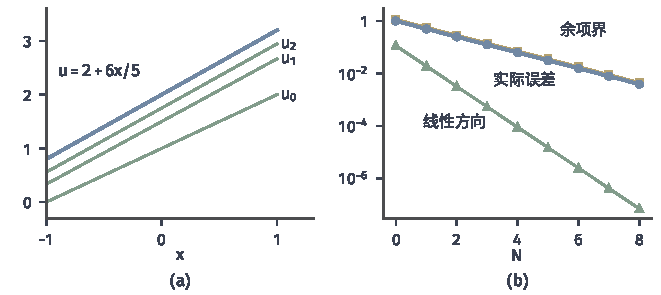
\includegraphics[width=112mm]{figures/04-spaces-measures-and-geometry/03-function-spaces/matplotlib/opeq-neumann-convergence/figure.pdf}
  \caption{$(I-\frac12T)u=1+x$的Neumann迭代。(a)绿色直线是迭代值$u_0,u_1,u_2$，蓝色直线是精确解。(b)对数纵轴上的误差：蓝色为实际误差，黄色为式~\eqref{eq:opeq-neumann-truncation}的上界，两者几乎平行；绿色为线性方向的误差，以$\frac16$的比率衰减，快于主导的常数方向。}
  \label{fig:opeq-neumann-convergence}
\end{BookInlineFigure}

\paragraph{小范数只是充分条件}
$\lvert\lambda\rvert\lVert K\rVert<1$保证可解，但远不是可解的必要条件。在秩二例子中取$\lambda=2$，常数方向的迭代系数满足$a_N=a+2a_{N-1}$，只要$a\neq0$就发散。可是$\lambda\neq1,3$，由式~\eqref{eq:opeq-rank-two-second}，方程对每个$f$仍有唯一解：
\[
  u=-a+3bx+r.
\]
取$f=1+x$，解为$u=-1+3x$。代回核对：$Tu=-1+x$，所以$u-2Tu=1+x$。方程可解与某种展开收敛是两件事。

反方向的例子是累积积分。$\lVert V\rVert=\sigma_1=2/\pi$，$\lambda=10$时$\lvert\lambda\rvert\lVert V\rVert>1$，定理的条件不成立，级数却仍然收敛。反复积分的公式是
\[
  (V^nf)(x)=\int_0^x\frac{(x-t)^{n-1}}{(n-1)!}f(t)\,\mathrm dt.
\]
由Cauchy--Schwarz不等式，$\lVert V^n\rVert\leq1/(n-1)!$，分母的增长压过任何$\lvert\lambda\rvert^n$。

所以$(I-\lambda V)u=f$对每个$\lambda$都有唯一解。取$f=1$，由$V^n1=x^n/n!$，得到
\[
  u(x)=\sum_{n=0}^\infty\frac{(\lambda x)^n}{n!}=e^{\lambda x}.
\]
$\lambda=10$时代回核对：$10Vu=e^{10x}-1$，所以$u-10Vu=1$。这与第~\ref{chap:operator-spectra}章的结论相符：$V$的谱只有$\{0\}$，没有非零特征值。要对所有参数判断可解性，需要用到$K$的紧性，这就是下一小节的内容。

\subsection{Fredholm可解条件}
\label{sec:opeq-fredholm}

先把参数分成情形。$\lambda=0$时方程就是$u=f$，总有唯一解。$\lambda\neq0$时，
\[
  I-\lambda K=-\lambda\Bigl(K-\frac1\lambda I\Bigr),
\]
所以齐次方程$(I-\lambda K)u=0$有非零解，当且仅当$1/\lambda$是$K$的特征值。

方阵有一个熟悉的事实：$\bm B\bm x=\bm 0$只有零解，当且仅当$\bm B\bm x=\bm b$对每个右端有解；若有非零解，则$\bm b$必须与$\bm B^\top$的零空间正交。下面说明，对$B=I-\lambda K$这个结论原样成立。先在紧自伴情形用特征方向看清答案，再对一般紧算子给出证明。

\paragraph{紧自伴情形的方向解释}
设$K$为紧自伴算子。为避免与参数$\lambda$混淆，记它的非零特征值为$\mu_j$。由第~\ref{chap:operator-spectra}章的谱分解，存在实数$\mu_j\neq0$与标准正交特征向量$e_j$，使每个$w\in H$写成$w=w_0+\sum_j\langle e_j,w\rangle e_j$，其中$w_0\in\ker K$；若特征值有无穷多个，则$\mu_j\to0$。把$I-\lambda K$作用在$u$上，得到
\[
  (I-\lambda K)u=u_0+\sum_j(1-\lambda\mu_j)\langle e_j,u\rangle e_j.
\]
$I-\lambda K$在零空间上是恒等作用，在第$j$个特征方向上乘以$1-\lambda\mu_j$。

若$\lambda$不等于任何$1/\mu_j$，这些乘子都不为零。又因为$\mu_j\to0$，乘子趋于$1$，只有有限个乘子离$1$较远，所以$\inf_j\lvert1-\lambda\mu_j\rvert>0$。逐方向除以乘子就得到有界逆：
\begin{equation}
  u=f_0+\sum_j\frac{\langle e_j,f\rangle}{1-\lambda\mu_j}e_j,
  \label{eq:opeq-self-adjoint-solution}
\end{equation}
其中$f_0$是$f$在$\ker K$上的分量。

若$\lambda=1/\mu_k$，乘子在$\mu_k$的特征空间上为零。这个特征空间有限维，就是齐次方程的解空间。此时方程可解，当且仅当$f$在这些方向上的系数为零，即$f\perp\ker(I-\lambda K)$；解可以加上该特征空间中的任意元素。

秩二例子中，$\lambda=1$时方程$(I-T)u=f$可解当且仅当$a=\langle1,f\rangle=0$。此时由式~\eqref{eq:opeq-rank-two-second}，第二个方程给出$\frac23\beta=b$，解为
\[
  u=c+\frac32bx+r,\qquad c\text{任意}.
\]
图~\ref{fig:opeq-fredholm-alternative}(a)画出三个乘子随$\lambda$的变化。除$\lambda=1,3$这两个参数外方程总是唯一可解，$\lambda=\frac12$与$\lambda=2$都在这个范围内，虽然只有前者满足小范数条件。

\begin{BookInlineFigure}
  \centering
  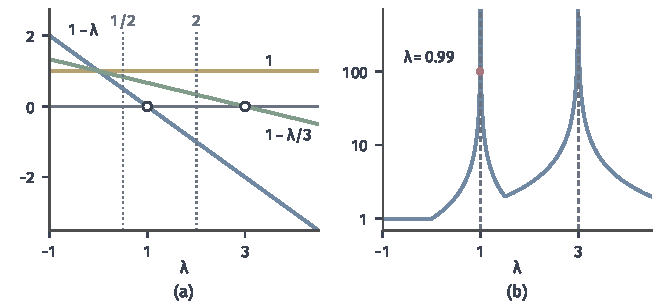
\includegraphics[width=112mm]{figures/04-spaces-measures-and-geometry/03-function-spaces/matplotlib/opeq-fredholm-alternative/figure.pdf}
  \caption{第二类方程$(I-\lambda T)u=f$对参数的依赖（核$1+xz$，测度$\mathrm dz/2$）。(a)三个方向的乘子：蓝色$1-\lambda$、绿色$1-\lambda/3$、黄色恒为$1$。空心圆处乘子为零，是例外参数；点线标出$\lambda=\frac12$（满足小范数条件）与$\lambda=2$（不满足，但仍唯一可解）。(b)逆算子的范数，对数纵轴，在两个例外参数处趋于无穷；红点为$\lambda=0.99$，范数$100$。}
  \label{fig:opeq-fredholm-alternative}
\end{BookInlineFigure}

\paragraph{Fredholm择一}
一般紧算子没有正交特征基可用，但结论的形式保持不变，只是正交条件要改用伴随方程的零空间。

\begin{theorem}[Fredholm择一]
\label{thm:opeq-fredholm}
设$H$为Hilbert空间，$K:H\to H$为紧算子，$\lambda\in\mathbb F$，$B=I-\lambda K$。则
\begin{enumerate}
  \item $\ker B$与$\ker B^*$都是有限维的，且$\dim\ker B=\dim\ker B^*$；
  \item $\operatorname{Ran}B$是闭子空间，因而$\operatorname{Ran}B=(\ker B^*)^\perp$；
  \item $\ker B=\{0\}$当且仅当$\operatorname{Ran}B=H$，此时$B^{-1}$有界。
\end{enumerate}
因此以下两种情形恰有一种成立。或者齐次方程$Bu=0$只有零解，此时对每个$f\in H$，方程$Bu=f$有唯一解，解由有界算子$B^{-1}$给出。或者齐次方程有非零解，此时$Bu=f$可解当且仅当$f\perp\ker B^*$，全部解为一个特解加上有限维子空间$\ker B$中的任意元素。
\end{theorem}

这一结论称为\term{Fredholm择一}（Fredholm alternative）。其中$B^*=I-\overline\lambda K^*$。取伴随方程$B^*w=0$的解空间的一组基$w_1,\ldots,w_r$，可解条件就是有限个等式
\begin{equation}
  \langle w_i,f\rangle=0,\qquad i=1,\ldots,r,
  \label{eq:opeq-compatibility}
\end{equation}
称为方程的\term{相容条件}（compatibility condition）。非唯一来自有限维的$\ker B$，不可解来自数据违反有限个相容条件，满足这些条件的数据都可解。

定理的关键是第二条。像的闭性由紧性事先保证，所以正交条件$f\perp\ker B^*$判断的是精确可解，而不只是$f$能否被输出逼近。上一节的对角算子$A$正好相反：每个数据都满足正交条件，但$A$的像不闭，$(1/n)$不在其中。

为什么条件要看伴随的零空间，而不是$\ker B$本身？用一个不自伴的例子说明。在$L^2(0,1)$上取秩一算子
\[
  (Ku)(x)=x\int_0^1u(z)\,\mathrm dz,
\]
并取$\lambda=2$，$B=I-2K$。

直接计算两个零空间。$u=x$满足$Ku=\frac12x$，所以$\ker B=\operatorname{span}\{x\}$。伴随是$(K^*w)(z)=\int_0^1xw(x)\,\mathrm dx$，输出总是常函数，代入$w=1$得$K^*1=\frac12$，所以$\ker B^*=\operatorname{span}\{1\}$。

把方程$u-2x\int_0^1u=f$两边在$[0,1]$上积分，左边是$\int u-2\cdot\frac12\int u=0$，所以
\[
  \int_0^1f(x)\,\mathrm dx=0
\]
是必要条件，这正是$f\perp1$，不是$f\perp x$。例如$f=2x-1$满足这个条件，全部解为$u=2x-1+cx$，而它与$x$并不正交，$\langle x,f\rangle=\frac16$。$f=1$违反条件，方程无解。

\paragraph{有限秩部分与小范数余项}
证明的想法是把紧算子拆成两部分：有限秩部分化成有限维线性方程组，余项用Neumann级数吸收。这样，无限维方程的可解性就完全由一个方阵决定。$\lambda=0$时$B=I$，结论直接成立，下面设$\lambda\neq0$。

\begin{proof}
第一步，分解。由第~\ref{chap:linear-operators}章，Hilbert空间上的紧算子能按算子范数被有限秩算子逼近。取有限秩算子$F$使$\lVert\lambda(K-F)\rVert<1$，记$C=I-\lambda(K-F)$。由定理~\ref{thm:opeq-neumann}，$C$有有界逆，于是
\[
  B=C-\lambda F=C(I-G),\qquad G=\lambda C^{-1}F.
\]

$G$仍是有限秩的有界算子。取$\operatorname{Ran}G$的一组基$b_1,\ldots,b_r$，则$Gu=\sum_{i=1}^r\ell_i(u)b_i$。系数$\ell_i$是有界线性泛函，因为有限维空间上的坐标泛函连续，与有界的$G$复合仍有界。由Riesz表示写成$\ell_i(u)=\langle a_i,u\rangle$，于是
\[
  Gu=\sum_{i=1}^r\langle a_i,u\rangle b_i.
\]

第二步，化为矩阵方程。令$\bm M$是$r\times r$矩阵，$\bm M_{i,j}=\langle a_i,b_j\rangle$，并记
\[
  \bm d(h)=(\langle a_1,h\rangle,\ldots,\langle a_r,h\rangle)^\top.
\]
我们断言：$(I-G)u=h$当且仅当$u=h+\sum_ic_ib_i$，其中$\bm c$满足
\[
  (\bm I-\bm M)\bm c=\bm d(h).
\]

若$(I-G)u=h$，则$u=h+Gu=h+\sum_ic_ib_i$，其中$c_i=\langle a_i,u\rangle$。把$u$的表达式代入这个内积，得到
\[
  c_i=\langle a_i,h\rangle+\sum_j\bm M_{i,j}c_j.
\]
反过来，若$\bm c$满足矩阵方程，令$u=h+\sum_jc_jb_j$，则
\[
  \langle a_i,u\rangle=\bm d(h)_i+(\bm M\bm c)_i=c_i,
\]
所以$Gu=\sum_ic_ib_i=u-h$。

第三步，像是闭的。由第二步，$h\in\operatorname{Ran}(I-G)$当且仅当$\bm d(h)\in\operatorname{Ran}(\bm I-\bm M)$。有限维子空间$\operatorname{Ran}(\bm I-\bm M)$是闭集，$\bm d$连续，所以$\operatorname{Ran}(I-G)$作为闭集的原像是闭的。$C$及其逆都连续，把闭集映成闭集，所以
\[
  \operatorname{Ran}B=C\bigl(\operatorname{Ran}(I-G)\bigr)
\]
闭。再由第~\ref{chap:linear-operators}章的关系$\overline{\operatorname{Ran}B}=(\ker B^*)^\perp$，第二条结论成立。

第四步，比较两个零空间的维数。取$h=0$，第二步说明$\bm c\mapsto\sum_ic_ib_i$是$\ker(\bm I-\bm M)$到$\ker(I-G)$的线性双射，这里用到$b_i$线性无关。$C$可逆，所以$\ker B=\ker(I-G)$，于是
\[
  \dim\ker B=\dim\ker(\bm I-\bm M).
\]

伴随一侧同样计算。由内积的共轭线性，$G^*w=\sum_i\langle b_i,w\rangle a_i$。若$w=G^*w$，令$d_i=\langle b_i,w\rangle$，则$w=\sum_jd_ja_j$，再与$b_i$作内积，得到
\[
  d_i=\sum_j\langle b_i,a_j\rangle d_j,
\]
这正是$\bm d=\bm M^{\mathsf H}\bm d$。反过来，每个满足此式的$\bm d$都给出$w=\sum_jd_ja_j\in\ker(I-G^*)$，且$w$确定$\bm d$，所以两个解空间线性同构。

又$B^*=(I-G^*)C^*$，$C^*$可逆，所以$\ker B^*$与$\ker(I-G^*)$维数相同。方阵与其共轭转置的秩相等，于是
\[
  \dim\ker B^*=\dim\ker(\bm I-\bm M^{\mathsf H})=\dim\ker(\bm I-\bm M)=\dim\ker B.
\]
这个公共的维数不超过$r$，第一条结论成立。

第五步，单射与满射等价。若$\ker B=\{0\}$，由第四步$\ker B^*=\{0\}$，再由第二条，$\operatorname{Ran}B=H$。反之，若$\operatorname{Ran}B=H$，则$\ker B^*=(\operatorname{Ran}B)^\perp=\{0\}$，由第四步$\ker B=\{0\}$。双射的有界算子$B$的逆有界，这由第~\ref{chap:linear-operators}章的开映射定理保证。
\end{proof}

用前面的秩一算子走一遍证明。这里$K$已是有限秩，取$F=K$，则$C=I$，$G=\lambda K$，只需一个基$b_1=x$，$a_1=\lambda\cdot1$（取实数$\lambda$），于是
\[
  \bm M=\langle a_1,b_1\rangle=\frac\lambda2,\qquad \bm d(h)=\lambda\int_0^1h.
\]
矩阵方程是一个标量方程：
\[
  \Bigl(1-\frac\lambda2\Bigr)c=\lambda\int_0^1h(x)\,\mathrm dx.
\]

$\lambda=1$时，$c=2\int h$，解为$u=h+2x\int_0^1h$。取$h=1$得$u=1+2x$，代回核对：$\int_0^1u=2$，所以$u-x\int_0^1u=1$。$\lambda=2$时，标量方程变成$0\cdot c=2\int h$，要求$\int h=0$，且$c$任意，这正是前面得到的相容条件和解的结构。

无限维方程的全部可解性就这样落在一个矩阵上，无限维的部分被可逆的$C$吸收了。这也说明了紧性的作用：若$K$不能被有限秩算子逼近，就无法这样把问题化到有限维。另一方面，定理只说明解存在并有界地依赖于数据，并不给出收敛的迭代格式，前面$\lambda=2$的例子正处于“唯一可解但Neumann级数发散”的情形。

定理的第三条也与第~\ref{chap:operator-spectra}章的结论一致：若$\mu\neq0$不是紧算子$K$的特征值，取$\lambda=1/\mu$，则$I-\lambda K$是单射，因而有有界逆，$K-\mu I=-\mu(I-\lambda K)$也有有界逆。所以紧算子的非零谱点都是特征值。这里的证明只用到有限秩逼近和Neumann级数，是这一事实的另一条论证路线。

\section{算子方程的稳定性}
\label{sec:opeq-stability}

前两节回答了解是否存在、是否唯一。实际数据总带有误差，即使方程对精确数据有唯一解，也还要问：数据改变一点，解会不会改变很多？这个问题只有在固定了输入和输出的范数之后才有确切含义，因为“一点”和“很多”都要用范数来量。本节先把三个要求并列写出，再分别考察第一类方程中的小奇异值和第二类方程中的共振参数。

\paragraph{适定问题}
设$X,Y$是赋范空间，$A:X\to Y$是有界线性算子，考虑方程$Ax=y$。按Hadamard的说法，若同时满足
\begin{enumerate}
  \item 存在：对每个$y\in Y$都有解；
  \item 唯一：解至多一个；
  \item 稳定：解连续依赖于数据，即$A^{-1}:Y\to X$连续，
\end{enumerate}
就称这个方程是\term{适定问题}（well-posed problem），否则称为\term{不适定问题}（ill-posed problem）。

三条要求相互独立，也都依赖于所取的范数。同一个求导问题，若把数据空间的范数加强到包含导数，误差放大就可能消失；所以说一个方程“不稳定”时，必须同时说明在哪对范数之下。$X,Y$都是Banach空间时，前两条已经蕴含第三条：有界双射的逆有界，这正是第~\ref{chap:linear-operators}章开映射定理的推论。因此在完备空间中，失去稳定性总是伴随着失去存在性，即像不是整个空间，甚至不闭。

\paragraph{趋于零的奇异值}
设$K:H_1\to H_2$为紧算子，并有无限多个正奇异值，$\sigma_j\to0$。在最小范数解的意义下，即使限制在可解的数据上，解也不连续依赖于数据。取数据扰动$\delta g_j=\sigma_ju_j$，则$\lVert\delta g_j\rVert=\sigma_j\to0$；它满足Picard条件，相应的最小范数解扰动为
\[
  \delta f_j=\frac{\langle u_j,\delta g_j\rangle}{\sigma_j}v_j=v_j,\qquad\lVert\delta f_j\rVert=1 .
\]
数据误差趋于零，解的误差却始终为$1$。所以映射$g\mapsto f^\dagger$在$\operatorname{Ran}K$上是无界的线性映射。

只有有限多个正奇异值时情况相反：Picard级数中各项都除以不小于$\sigma_{\min}$的数，所以$\lVert f^\dagger\rVert\leq\lVert g\rVert/\sigma_{\min}$，其中$\sigma_{\min}$是最小的正奇异值。秩二例子中$\sigma_{\min}=1/3$，误差至多放大三倍。误差放大的程度不由“算子是否可逆”这一定性性质决定，而由奇异值离零有多远决定。

\begin{theorem}[紧算子的像不闭]
\label{thm:opeq-compact-range}
设$K:H_1\to H_2$为紧算子，$\operatorname{Ran}K$是无限维的。则$\operatorname{Ran}K$在$H_2$中不闭，$K$限制在$(\ker K)^\perp$上的逆$\operatorname{Ran}K\to(\ker K)^\perp$无界。
\end{theorem}

\begin{proof}
先证逆无界。设逆有界，范数为$c$，则$\operatorname{Ran}K$中范数不超过$1$的元素都是$K$作用在$(\ker K)^\perp$中范数不超过$c$的元素上的像。$K$紧，这些像组成相对紧集，所以$\operatorname{Ran}K$中的每个有界序列都有在$H_2$中收敛的子列。但$\operatorname{Ran}K$是无限维子空间，由Gram--Schmidt过程可以在其中取一列标准正交向量，它们两两距离都是$\sqrt2$，没有收敛子列；这正是第~\ref{chap:functions-as-vectors}章所说的无限维闭球不紧。矛盾，所以逆无界。

再证像不闭。若$\operatorname{Ran}K$闭，它作为闭子空间是Hilbert空间，$K$限制在闭子空间$(\ker K)^\perp$上就是两个Hilbert空间之间的有界双射。由开映射定理，其逆有界，与上一段矛盾。
\end{proof}

结合上一节，无限秩紧算子的第一类方程三条要求全部失效：像不闭，存在性只对一个稠密而不闭的子空间成立；零空间可能非零；在像上解也不连续依赖于数据。对第一类方程，这种不适定不是例外情形，而是无限维紧算子的一般性质。

\paragraph{累积积分的误差放大}
对累积积分$V$，奇异值$\sigma_k=1/((k-\frac12)\pi)$按$1/k$衰减。取真解$f=1$，精确数据$g=Vf=x$。在数据上加入扰动$\delta u_{20}$，$\delta=0.01$，最小范数解多出$(\delta/\sigma_{20})v_{20}$，其范数为$19.5\pi\delta\approx0.61$，振幅$\sqrt2\times0.61\approx0.87$。图~\ref{fig:opeq-noise-amplification}中两条数据曲线几乎重合，解中却出现明显的快速振荡。

\begin{figure}[!htb]
  \centering
  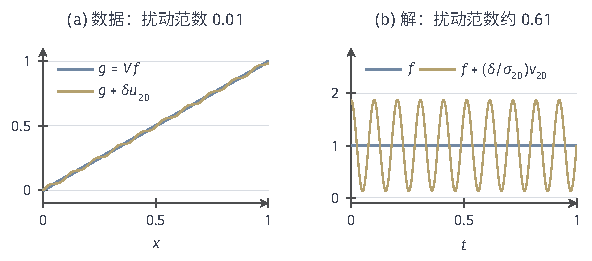
\includegraphics[width=100.2mm]{figures/02-abstract-mathematics/03-function-spaces/tikz/c3-noise-amplification/figure.pdf}
  \caption{第一类方程$Vf=g$（$(Vf)(x)=\int_0^xf$）中小奇异值放大扰动。真解$f=1$，数据$g=x$。(a)数据加上范数为$0.01$的扰动$\delta u_{20}$，与原数据几乎重合。(b)相应的最小范数解多出$(\delta/\sigma_{20})v_{20}$，振幅约$0.87$、范数约$0.61$，放大倍数$1/\sigma_{20}=19.5\pi\approx61$。}
  \label{fig:opeq-noise-amplification}
\end{figure}

这一机制与上一节“求解$Vf=g$就是求导”的结论是同一件事。$V$把快速振荡的输入平均掉，反解时必须把同样的振荡放大回去，振荡越快，放大倍数$1/\sigma_k=(k-\frac12)\pi$越大。求导在$L^2$范数下不连续：$\sin(n\pi x)/n$的范数趋于零，导数$\pi\cos(n\pi x)$的范数却不趋于零。

\paragraph{有限截断与误差的两部分}
一个自然的做法是只保留前$m$个奇异方向，令
\[
  f_m^\delta=\sum_{j\leq m}\frac{\langle u_j,g^\delta\rangle}{\sigma_j}v_j ,
\]
其中$g^\delta$是带误差的数据，$\lVert g^\delta-g\rVert\leq\delta$，$g=Kf^\dagger$为精确数据。这个截断算子有界，范数为$1/\sigma_m$。设$f_m$是用精确数据得到的截断解，则$f_m^\delta-f^\dagger=(f_m-f^\dagger)+(f_m^\delta-f_m)$。第一项是舍弃方向上的系数，第二项只含前$m$个方向上数据误差的放大；由Bessel不等式，
\begin{equation}
  \lVert f_m^\delta-f^\dagger\rVert\leq\Bigl(\sum_{j>m}\lvert\langle v_j,f^\dagger\rangle\rvert^2\Bigr)^{1/2}+\frac{\delta}{\sigma_m}.
  \label{eq:opeq-truncation-split}
\end{equation}

式~\eqref{eq:opeq-truncation-split}中，$m$增大使第一项减小、第二项增大。固定$m$时得到的是有界算子，所以截断本身是稳定的；但它求的不再是原方程的精确解，而且稳定常数$1/\sigma_m$随$m$变坏。因此不能从形式逆或某个有限截断直接推出可靠恢复：截断位置必须结合误差水平$\delta$和真解在高阶方向上的大小来选。这种选择以及用惩罚项代替硬截断的方法，属于正则化问题，可参考\BookChapterRef{chap:function-fitting-regularization}{卷五第10章“函数拟合与正则化”}；有限维中奇异值截断与条件数的关系，可参考\BookChapterRef{chap:solution-error-regularization}{卷二第14章“求解误差、正则化与方法选择”}。

\paragraph{第二类方程与共振参数}
第二类方程在$1/\lambda$不是特征值时有有界逆，因而是适定的。但“有界”并不说明界有多大。设$K$紧自伴，$\lambda$不是任何$1/\lambda_j$。由上一节的方向表示，$(I-\lambda K)^{-1}$在零空间上乘以$1$，在第$j$个特征方向上乘以$1/(1-\lambda\lambda_j)$，所以
\[
  \bigl\lVert(I-\lambda K)^{-1}\bigr\rVert=\max\Bigl\{\sup_j\frac{1}{\lvert1-\lambda\lambda_j\rvert},\ 1\Bigr\},
\]
其中$1$来自零空间上的恒等作用。$H$无限维而零空间为$\{0\}$时，特征值有无穷多个且趋于零，相应乘子的倒数趋于$1$，所以这一项不改变结果。$\lambda$靠近某个$1/\lambda_k$时，相应乘子的倒数趋于无穷，数据在$e_k$方向上的误差被放大$1/\lvert1-\lambda\lambda_k\rvert$倍。

秩二例子中，$\lVert(I-\lambda T)^{-1}\rVert=\max\{1/\lvert1-\lambda\rvert,1/\lvert1-\lambda/3\rvert,1\}$。$\lambda=0.99$时这个范数为$100$：源项在常数方向上$10^{-3}$的误差，会使解在同一方向上改变$0.1$，而其他方向上的误差几乎不被放大。与第一类方程比较，第二类方程的敏感性集中在共振参数附近的有限个方向上，远离这些参数时有统一的界；第一类方程的敏感性则来自无穷多个趋于零的奇异值，任何参数都无法消除。

\paragraph{算子的扰动}
实际计算中，算子本身也常被近似，例如用有限秩核代替原来的积分核。Neumann级数给出这时的稳定性判据。设$B=I-\lambda K$有有界逆，$E$是有界算子，且$\lVert B^{-1}\rVert\lVert E\rVert<1$。写成$B+E=B(I+B^{-1}E)$，由定理~\ref{thm:opeq-neumann}，$I+B^{-1}E$可逆，于是$B+E$可逆且
\[
  \bigl\lVert(B+E)^{-1}\bigr\rVert\leq\frac{\lVert B^{-1}\rVert}{1-\lVert B^{-1}\rVert\lVert E\rVert}.
\]
若$K_m$是$K$的有限秩近似，取$E=-\lambda(K_m-K)$，只要$\lvert\lambda\rvert\lVert K-K_m\rVert\lVert B^{-1}\rVert<1$，近似方程就仍然唯一可解，并有可控的稳定常数。这一条件同时依赖近似误差和$\lVert B^{-1}\rVert$：参数越靠近共振值，对算子近似的精度要求越高。

对第一类方程，同样的论证无法进行，因为$K$本身没有有界逆可以作为起点。这再次说明两类方程的区别来自恒等项的结构：恒等项提供了一个可逆的主部，紧算子只是对它的扰动；第一类方程中紧算子就是全部，它的逆的不连续性无法通过细化近似消除。

\section{本章小结}
\label{sec:opeq-summary}

本章开头问了三件事：给定输出能否由某个输入产生，输入是否唯一，数据误差会怎样影响解。对第一类方程$Kf=g$，前两个问题分别由像和零空间回答：有解当且仅当$g\in\operatorname{Ran}K$，解集是一个特解加上$\ker K$。紧算子的奇异系统把这两个条件写成系数条件。$g\perp\ker K^*$只说明$g$落在像的闭包里，还要求Picard条件$\sum_j\lvert\langle u_j,g\rangle\rvert^2/\sigma_j^2<\infty$，形式逆系数才拼成输入空间的元素；此时最小范数解$f^\dagger$是全部解中与零空间正交的那一个。累积积分$V$把这些条件落到具体函数上：常函数$1$能被输出任意逼近却不在像中，像中的数据恰是在$0$处取零且导数平方可积的函数，解就是导数。

第二类方程$(I-\lambda K)u=f$多了一个恒等项，在$K$看不见的方向上保留了信息。$\lvert\lambda\rvert\lVert K\rVert<1$时，Neumann级数直接给出有界逆，截断余项按$\lvert\lambda\rvert\lVert K\rVert$的幂几何下降；这一条件只是充分的，秩二例子中$\lambda=2$时级数发散而方程唯一可解。对一般参数，Fredholm择一说明：齐次方程只有零解时方程对一切数据唯一可解且逆有界；否则零空间有限维，可解性由有限个相容条件$\langle w_i,f\rangle=0$决定，其中$w_i$张成伴随方程的零空间。紧性使$I-\lambda K$的像闭，这是第二类方程与第一类方程的根本差别。

关于稳定性，适定性要求存在、唯一和连续依赖三条同时成立，并且依赖所取的范数。无限秩紧算子的像不闭，在像上求逆无界：数据扰动$\sigma_ju_j$趋于零，解的扰动始终为单位长度，累积积分中这就是求导的不稳定。截断到前$m$个奇异方向得到有界的近似逆，误差分为舍弃方向上的偏差和至多$\delta/\sigma_m$的噪声放大两部分，所以形式逆和固定截断都不能直接当作可靠恢复。第二类方程远离共振参数时是适定的，敏感性只在$\lambda$接近某个$1/\lambda_k$时出现，并集中在有限个方向上；在这种情形下，算子的小扰动也可以由Neumann级数控制。

本章只确定了方程何时可解、解怎样依赖数据。怎样根据误差水平选择截断位置或惩罚强度，怎样设计求解算法并比较偏差与误差放大，由卷五的正则化与函数拟合承担。下一章转向另一类有限表示问题：不是从输出反推输入，而是用有限个简单函数去接近给定的目标函数，并比较不同表示预算下的最佳误差。

